\section{Результаты}
Замеры времени работы программы с разным количеством процессов и разным размером сетки. Сетка имеет размер $n \times n \times n$.

\resizebox{\columnwidth}{!}{
\begin{tabular}{|c|c|c|c|c|c|c|c|c|}
\hline
Кол-во процессов& $n = 12$, мс & $n = 24$, мс & $n = 48$, мс & $n = 96$, мс & $n = 144$, мс \\
\hline
1, без MPI & 0.911 & 24.122 & 639.690 & 17232.042 & 70445.164 \\
\hline
2 & 0.927 & 14.587 & 369.080 & 9146.040 & 38472.441 \\
\hline
3 & 1.203 & 11.756 & 201.487 & 6332.821 & 27606.756 \\
\hline
4 &1.125 & 11.698 & 270.489 & 4816.114 & 21962.017 \\
\hline
6 &2.112 & 13.897 & 204.099 & 4338.967 & 19534.214 \\
\hline
8 & 2.643 & 13.243 & 252.020 & 4182.772 & 20196.098\\
\hline
12 & 5.036 & 15.314 & 183.897 & 3427.126 & 19790.645 \\
\hline
16 & 22904.747 & 65687.236 & $> 120$ сек & $> 120$ сек & $> 120$ сек \\
\hline
\end{tabular}
}

\section{Визулизация результата}
\begin{center}
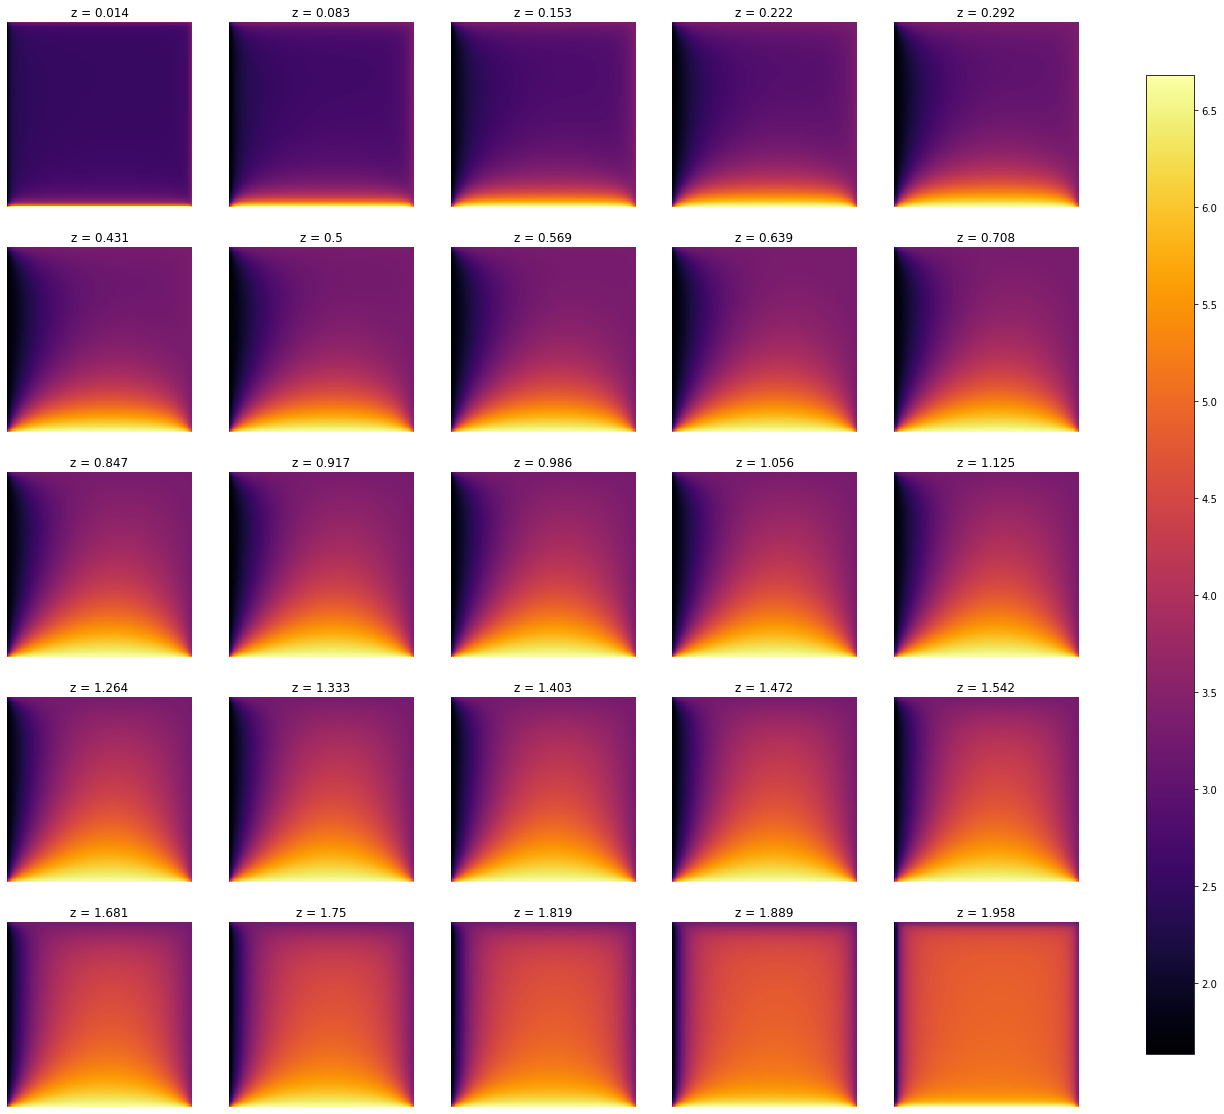
\includegraphics[width=\textwidth]{images/heatmap.png}\newline\noindent
\end{center}
Размеры области:$l_x = 2, l_y = 2, l_z = 2$.

Начальные условия: $u_{down} = 3, u_{up} = 7, u_{left} = 2, u_{right} = 5, u_{front} = 1, u_{back} = 3$.
\pagebreak